Tato kapitola pojednává o~obecném popisu dopravního značení, jehož automatizované rozpoznání pomocí počítače je cílem této práce. Dále jsou v~této kapitole popsány běžně používané metody pro detekci a~klasifikaci dopravního značení v~současné době, a~také metriky používané pro vyhodnocení úspěšnosti v~oboru detekce objektů. Nakonec jsou zmíněny zajímavé existující práce z~této oblasti, jimi použité metody a~dosažené výsledky.


%%%%%%%%%%%%%%%%%%%%%%%%%%%%%%%%%%%%%%%%%%%%%%%%%%%%%%%%%%%%%%%%%%%%%%%%%%%%%%%%%%%%%%%%%%%


\section{Dopravní značení}
\label{dopravniZnaceni}
Dopravní značení slouží k~účelu řízení a~regulace dopravy na pozemních komunikacích a~tedy k~zajištění plynulosti a~bezpečnosti dopravy. Svislé dopravní značení, kterému se tato práce věnuje, se běžně nachází na stranách silnice či na konstrukci nad silnicí \cite{dopravniZnacka, dopravniZnaceniVCesku}.

\subsection*{Dělení dopravního značení v~Česku}
\label{dopravniZnaceniDeleni}
Dělení svislého dopravního značení, které je nejčastějším způsobem dopravního značení, se skládá ze šesti tříd vizualizovaných na obrázku \ref{kolazDopravniZnacky} a~jejich krátký popis podle \cite{seznamDopravnichZnacek, dopravniZnacka, dopravniZnaceniVCesku} je následovný:

\begin{itemize}
    \item \textbf{Výstražné dopravní značky} upozorňují účastníky silničního provozu na možná nebezpečí a~rizika. Jsou to zpravidla trojúhelníky s~bílým pozadím, piktogramem uprostřed a~ohraničené červenou barvou.
    \item \textbf{Značky upravující přednost} se používají na křižovatkách pro určení přednosti. Tyto značky mohou být trojúhelníkové, čtvercové i~osmiúhelníkové a~barevné provedení je buďto žluté, červené či modré.
    \item \textbf{Zákazové dopravní značky} ukládají účastníkům silničního provozu zákazy jistých činností.
    \item \textbf{Příkazové dopravní značky} slouží k~odstranění možnosti vzniku nebezpečných situací. Tyto značky jsou vždy kruhového tvaru s~modrým barevným provedením a~bílým piktogramem či textem uprostřed.
    \item \textbf{Informativní dopravní značky} poskytují pro účastníky silničního provozu důležité informace, určující například orientaci, typ zóny či silnice.
    \item \textbf{Dodatkové tabulky} slouží k~doplnění či omezení významu jiných dopravních značek. 
\end{itemize}

\begin{figure}[H]
    \centering
    \tmpframe{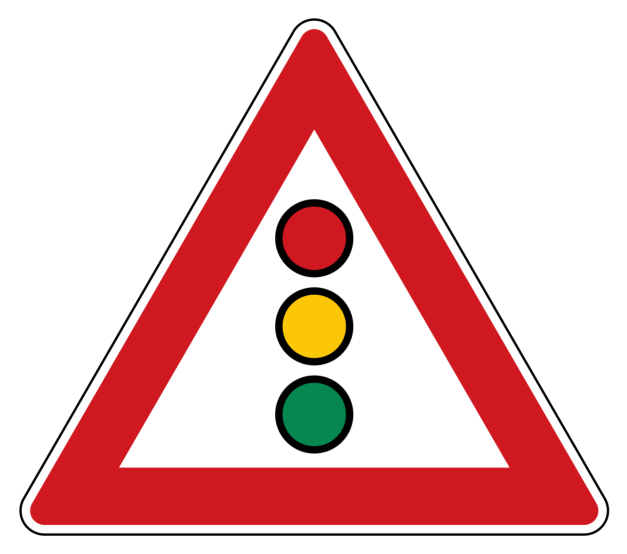
\includegraphics[width=0.15\linewidth]{figures/znacky/vystrazne.eps}}
    \tmpframe{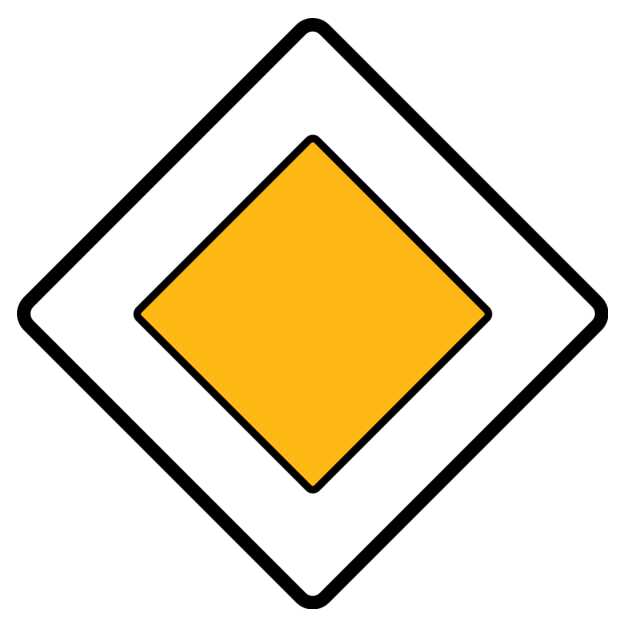
\includegraphics[width=0.15\linewidth]{figures/znacky/prednost}}
    \tmpframe{
\includegraphics[width=0.15\linewidth]{figures/znacky/zakazove}}
    \tmpframe{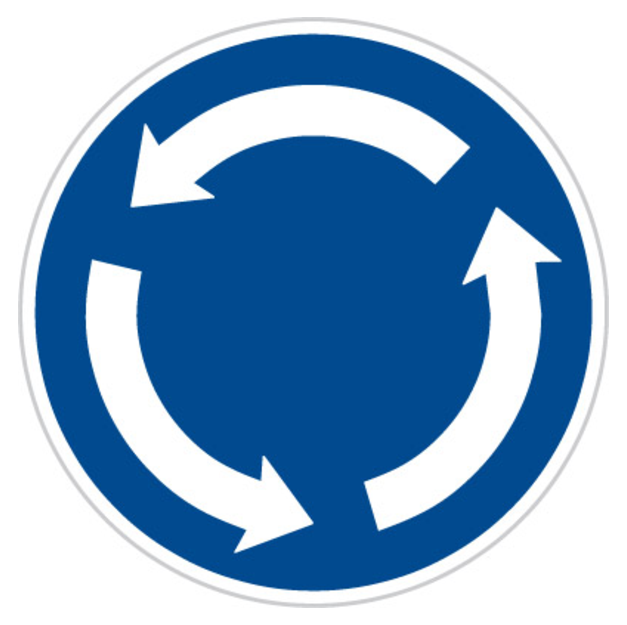
\includegraphics[width=0.15\linewidth]{figures/znacky/prikazove}}
    \tmpframe{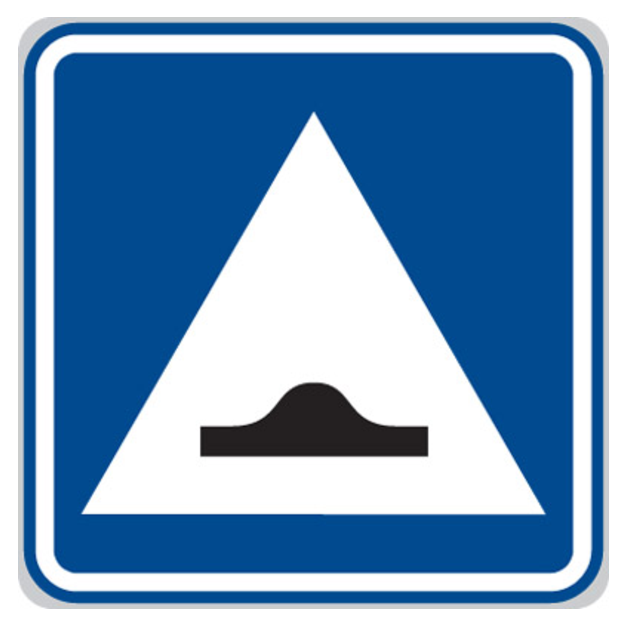
\includegraphics[width=0.15\linewidth]{figures/znacky/informativni}}
    \tmpframe{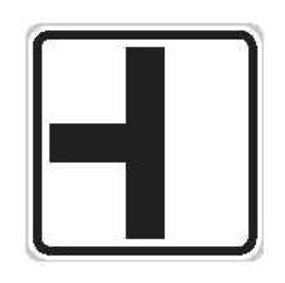
\includegraphics[width=0.15\linewidth]{figures/znacky/dodatkove}}
    \caption{Příklad značek jednotlivých tříd.\footnotemark}
    \label{kolazDopravniZnacky}
\end{figure}

\footnotetext{Převzato z~\cite{seznamDopravnichZnacek}.}

\subsection*{Vzhled dopravních značek}
\label{dopravniZnaceniBarvy}
Evropská norma definuje základní vlastnosti značek, ale ponechává státům jistou volnost. Značky v~jednotlivých státech se mohou trochu lišit, ať už barvou, velikostí či tvarem. Pro člověka je tento rozdíl téměř nevnímatelný, ale počítači může při detekci působit potíže. Na obrázku \ref{kolazStopky} lze vidět variabilitu barev a~způsobu zpracování značek \emph{stop} pěti Evropských států (Rakouska, Česka, Řecka, Rumunska a~Turecka) \cite{dopravniZnacka}.

\begin{figure}[H]
    \centering
    \tmpframe{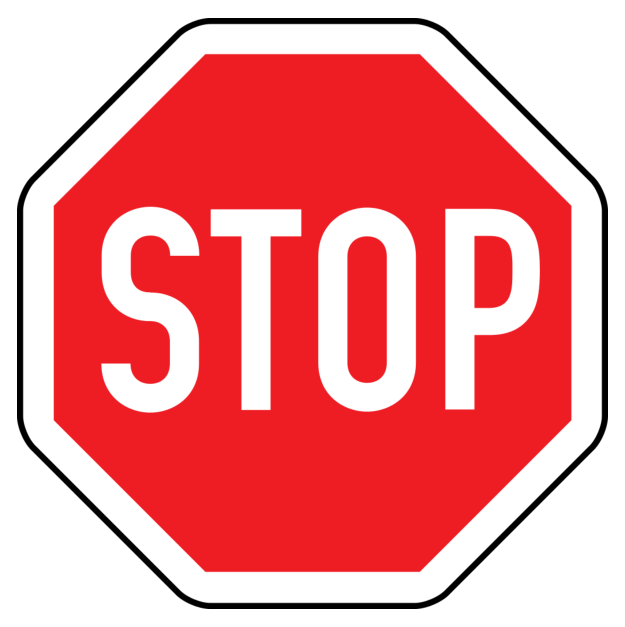
\includegraphics[width=0.19\linewidth]{figures/znacky/rakouske}}\hfill
    \tmpframe{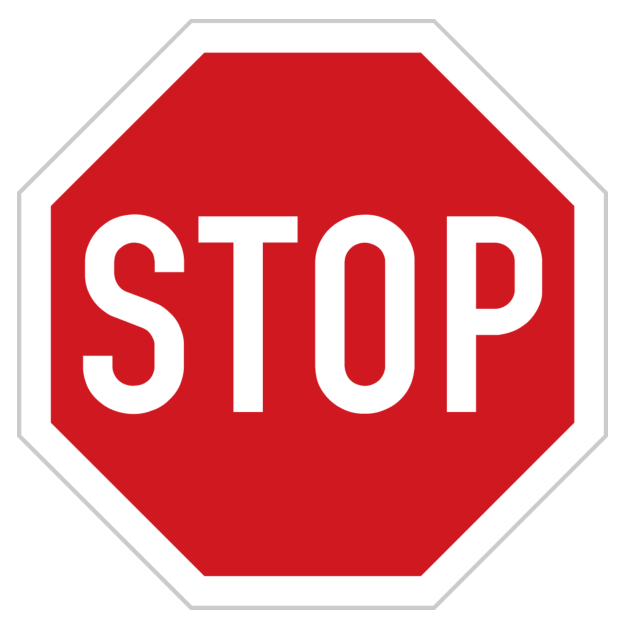
\includegraphics[width=0.19\linewidth]{figures/znacky/ceske}}\hfill
    \tmpframe{
\includegraphics[width=0.19\linewidth]{figures/znacky/recke}}\hfill
    \tmpframe{
\includegraphics[width=0.19\linewidth]{figures/znacky/rumunske}}\hfill
    \tmpframe{
\includegraphics[width=0.19\linewidth]{figures/znacky/turecke}}
    \caption{Rozdílnost značek stop některých Evropských zemí.\footnotemark}
    \label{kolazStopky}
\end{figure}

\footnotetext{Převzato z~\url{https://en.wikipedia.org/wiki/Comparison_of_European_road_signs}}

Ačkoli se detekce dopravních značek může zdát jako jednoduchá úloha, tak stále není úplně vyřešena a~stále přibývají kvalitní práce posouvající tuto problematiku kupředu. Velký problém při detekci značek sehrávají různé světelné podmínky, přírodní vlivy (např. vyblednutí barev, sníh, déšť), vandalismus, deformace či jiné poškození značek, částečné překrytí, malá velikost, apod., jak lze vidět na obrázku \ref{fig:kolazZnacky}.

\begin{figure}[H]
    \centering
    \tmpframe{\includegraphics[width=0.20\linewidth]{figures/detekce/bad_conditions/bad_sign_1.png}}\hfill
    \tmpframe{\includegraphics[width=0.20\linewidth]{figures/detekce/bad_conditions/bad_sign_2.png}}\hfill
    \tmpframe{\includegraphics[width=0.20\linewidth]{figures/detekce/bad_conditions/bad_sign_3.png}}\hfill
    \tmpframe{\includegraphics[width=0.20\linewidth]{figures/detekce/bad_conditions/bad_sign_4.png}}\\
    \tmpframe{\includegraphics[width=0.20\linewidth]{figures/detekce/bad_conditions/bad_sign_5.png}}\hfill
    \tmpframe{\includegraphics[width=0.20\linewidth]{figures/detekce/bad_conditions/bad_sign_6.png}}\hfill
    \tmpframe{\includegraphics[width=0.20\linewidth]{figures/detekce/bad_conditions/bad_sign_7.png}}\hfill
    \tmpframe{\includegraphics[width=0.20\linewidth]{figures/detekce/bad_conditions/bad_sign_8.png}}
    \caption{Problémové dopravní značky pocházející z použité datové sady.}
    \label{fig:kolazZnacky}
\end{figure}

%%%%%%%%%%%%%%%%%%%%%%%%%%%%%%%%%%%%%%%%%%%%%%%%%%%%%%%%%%%%%%%%%%%%%%%%%%%%%%%%%%%%%%%%%%%

\section{Způsoby detekce dopravního značení}
\label{zpusobyDetekce}
Při detekci těchto objektů lze vycházet z~jejich specifického tvaru, barvy a~také jejich dobré rozlišitelnosti od pozadí \cite{tsDetectOverview}. Vzhledem k~množství již existujících prací na toto téma se nabízí celá řada způsobů, jak k~řešení tohoto problému přistupovat, proto zde bude zmíněno jen několik nejdůležitějších. Problém lze řešit také pomocí konvolučních neuronových sítí, popsaných samostatně v~kapitole \ref{detekceKonv}. Na rozdíl od klasifikace objektů, jejich detekce vyžaduje lokalizaci (běžně více) objektů v~rámci celého snímku \cite{rcnn}.

\subsection*{Segmentace na základě barvy}
\label{zpusobyDetekceSegmentace}
Základní segmentace obrazu je běžně dosažena pomocí prahování na základě určité barvy. Podle práce \cite{tsDetect} je intuitivní použití barevného modelu RGB (red, green, blue), u~kterého je každý pixel definován pomocí třech hodnot: červené, zelené a~modré. Prahování pomocí tohoto barevného modelu lze vyjádřit pomocí rovnic \eqref{eq:soustavaRGB1} a~\eqref{eq:soustavaRGB2}.
\begin{align}
    \label{eq:soustavaRGB1}
    g(x,y) &= k_1\begin{cases}
    \ R_a \leq f_r(x,y) \leq R_b\\
    \ G_a \leq f_g(x,y) \leq G_b\\
    \ B_a \leq f_b(x,y) \leq B_b\end{cases}\\
    \label{eq:soustavaRGB2}
    g(x,y) &= k_2 \text{ v~jakémkoli jiném případě}
\end{align}
Funkce $f_*(x,y)$ udávají hodnotu jednotlivých barevných složek daného bodu obrázku. Výsledný pixel nabývá hodnoty $k_1$ pouze v~případě, že všechny barevné kanály pixelu spadají do předem definovaných intervalů, jinak nabývá hodnoty $k_2$. Velkou nevýhodou tohoto barevného modelu ovšem je, že je velmi citlivý na změnu osvětlení. Z~tohoto důvodu se již v~75. letech minulého století zavedly nové barevné modely HS* (HSI, HSV, HSL), které jsou mnohem bližší lidskému vnímání barev \cite{tsDetectOverview}. První složka je \emph{hue}, tedy odstín. Druhá je \emph{saturation}, která udává sytost a~poslední např. \emph{intensity} (I), udávající intenzitu barvy. Převod z~barevného prostoru RGB, pomocí něhož jsou obrázky běžně reprezentovány, do jednoho ze zmíněných modelů byl v~minulosti výpočetně dosti náročný, ale s~dnešní výpočetní kapacitou to není problém, a~proto se často využívá. Převod z~barevného prostoru RGB do HSV podle \cite{tsRychlaDetekce} je následující:
\begin{align}
    \label{eq:soustavaHSV}
    V~&= max(R,G,B)\\
    S~&= \begin{cases}
    \ \frac{V~- min(R,G,B)}{V}  & V~\neq 0\\
    \ 0 & V~= 0\end{cases}\\
    H &= \begin{cases}
    \ \frac{60(G-B)}{V - min(R,G,B)} & V~= R \vspace{4px}\\
    \ \frac{120+60(B-R)}{V - min(R,G,B)} & V~= G\vspace{4px}\\
    \ \frac{240+60(R-G)}{V - min(R,G,B)} & V~= B\end{cases}
\end{align}
Z~tabulky porovnání detekčních metod v~\cite{tsDetectOverview} vyplývá, že je používaný jak barevný model RGB, použit $5\times$, tak barevný model HS*, použit také $5\times$. Mimo ně byl v~porovnání jedenkrát uveden model CIECAM97. Příklad použití prahování na základě červené barvy při použití modelu RGB lze vidět na obrázku~\ref{fig:prahovani}.

\begin{figure}[H]
    \centering
    \tmpframe{\includegraphics[width=0.495\linewidth]{figures/detekce/TS.png}}\hfill
    \tmpframe{\includegraphics[width=0.495\linewidth]{figures/detekce/TS_thresholding.png}}
    \caption{Prahování na základě červené barvy pomocí barevného modelu RGB. Upraveno pomocí \texttt{OpenCV}.}
    \label{fig:prahovani}
\end{figure}


\subsection*{Cannyho hranový detektor}
\label{zpusobyDetekceCanny}
Tento detektor byl vytvořen v~roce 1986 Johnem Cannym, ale ještě dnes se v~oblasti zpracování obrazu hojně využívá \cite{canny}. Canny definoval základní pravidla, která musí detektor splňovat, a~ty jsou následovné:

\begin{enumerate}
    \item \textbf{Vysoká úroveň detekce}. Detektor by měl mít nízkou pravděpodobnost selhání detekce existující hrany a~zároveň nízkou pravděpodobnost detekce neexistující hrany.
    \item \textbf{Dobrá lokalizace}. Body označené jako hraniční by měly být co nejblíže středu reálné hrany.
    \item \textbf{Pouze jedna detekce jedné hrany}. Pokud je jedna hrana detekována vícekrát, pouze jedna z~těchto detekcí by měla být označena jako správná a~ostatní ignorovány.
\end{enumerate}

\begin{figure}[H]
    \centering
    \tmpframe{\includegraphics[width=0.495\linewidth]{figures/detekce/TS.png}}\hfill
    \tmpframe{\includegraphics[width=0.495\linewidth]{figures/detekce/TS_canny.png}}
    \caption{Detekce hran pomocí Cannyho hranového detektoru. Upraveno pomocí \texttt{OpenCV}.}
    \label{fig:canny}
\end{figure}


Algoritmus je koncipován pouze pro práci se signálem obsahující jeden kanál, proto nelze metodu přímo použít například na RGB obrázek, který má tři kanály. První je potřeba převést obrázek do stupňů šedi. Výsledek detekce hran dopravní značky pomocí Cannyho detektoru lze vidět na obrázku \ref{fig:canny}. Obecný popis zpracování obrazového signálu Cannyho detektorem je následovný \cite{canny, tsRychlaDetekce, tsWindowsPhone}.

\begin{enumerate}
    \item Redukce šumu  -- provedení konvoluce obrazu $f$ s~gaussovým filtrem $G$, tedy $f * G$.
    \item Nalezení velikosti a~směru gradientu. $n$ by měla být orientovaná normála ke směru detekované hrany a~i~přesto, že tento směr není znám, je možné udělat jeho poměrně přesný odhad na základě směru vyhlazeného gradientu:
    \begin{align}
        \label{eq:soustavaCanny}
        n &= \frac{\nabla(G * f)}{|\nabla(G * f)|}
    \end{align}
    \item Nalezení správné pozice hrany pomocí operace zvané \emph{nonmaximum suppression}, tedy potlačení ne-maximálních hodnot. Ta slouží k~odstranění hodnot, které nejsou ve směru gradientu lokální maxima.
    \item Provést v~obraze prahování s~hysterezí pro odstranění bezvýznamných hran. Existují dva zadané prahy $T_1$ (minimální) a~$T_2$ (maximální). Pokud je odezva v~bodě vyšší než $T_2$, je bod označen za součást hrany. Pokud se odezva bodu nachází mezi $T_1$ a~$T_2$ a~zároveň je spojena s~bodem, který již byl označen jako součást hrany, je tento bod také označen za součást hrany. Všechny ostatní body jsou označeny tak, že nejsou považovány za součást žádné hrany.
\end{enumerate}

Velkou výhodou Cannyho detektoru hran je, že není citlivý na šum a~dokáže tedy pracovat se značně zašuměným obrazem \cite{tsDetekceTapuska}.


\subsection*{Detekce geometrických tvarů v~obraze pomocí Houghovy transformace}
\label{zpusobyDetekceHough}
Houghova transformace je výpočetně poměrně náročná operace, a~proto se na obraz běžně první aplikuje hranový detektor a~až poté se provádí Houghova transformace. Detekce hran vede k~poměrně značné redukci informace a~šumu v~obrazu a~zachová informaci potřebnou pro nalezení objektu. Proto podstatně zrychluje celý proces a~zpřesňuje výsledek. Pomocí Houghovy transformace se hledají tzv. ROI (\emph{Regions of Interest}, tedy oblasti zájmu), ve kterých se může dopravní značka nacházet. Metoda byla nesčetněkrát modifikována a~rozšířena~\cite{houghTransformace, tsDetekceSvoboda}.

\subsubsection{Klasická Houghova transformace}
\label{zpusobyDetekceHoughtKlasicka}
Houghova transformace pro detekci přímek vychází z~rovnice přímky \eqref{eq:rovnicePrimky}. Podle \cite{houghTransformace, tsWindowsPhone} libovolná přímka může být reprezentována pomocí jediného bodu v~prostoru. Parametr $\theta$ udává úhel, který svírá normála přímky s~kladnou částí osy $x$. Parametr $\rho$ udává vzdálenost přímky od středu souřadného systému.
\begin{align}
    \label{eq:rovnicePrimky}
    x \cos{\theta} + y \sin{\theta} = \rho
\end{align}
Tyto parametry je pro detekci přímky potřeba nalézt a~vytváří se pro tyto účely dvou-dimenzionální Houghův prostor složený z~parametrů $\theta$ a~$\rho$. Postupně se prochází celý prohledávaný prostor a~pro každý bod se určí všechny možné přímky procházející tímto bodem a~umístí se do zmíněného Houghova prostoru. Pro daný bod tedy vznikne sinusoida, viz obrázek \ref{fig:hough}. Sinusoidy všech bodů, které leží na stejné přímce, se protnou ve stejném bodě.

\begin{figure}[H]
    \centering
    \tmpframe{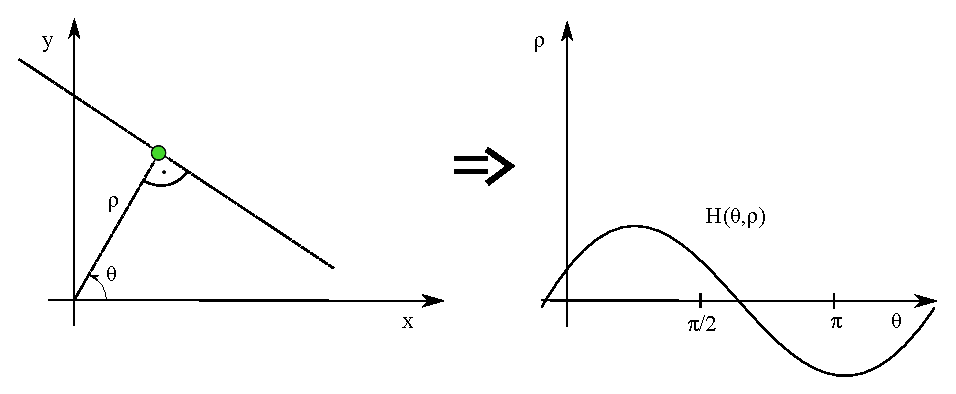
\includegraphics[width=0.9\linewidth]{figures/detekce/hough.eps}}
    \caption{Bod obrázku převedený na sinusoidu v~Houghově prostoru.}
    \label{fig:hough}
\end{figure}

\subsubsection{Zobecněná Houghova transformace}
\label{zpusobyDetekceHoughtZobecnena}
Stejně jako metoda pro detekci přímek vycházela z~rovnice přímky \eqref{eq:rovnicePrimky}, vychází metoda pro detekci kružnic z~rovnice kružnice \eqref{eq:rovniceKruznice}, kde $a$ a~$b$ udávají střed kružnice a~parametr $c$ udává poloměr kružnice.
\begin{align}
    \label{eq:rovniceKruznice}
    (x - a)^2 + (y - b)^2 = c
\end{align}
Postupuje se stejně jako u~detekce přímek, pouze jsou zde hledány tři parametry, a~proto Houghův prostor bude mít v~tomto případě tři dimenze.

\subsection*{Histogram orientovaných gradientů}
Při studiu této problematiky jsem vycházel z~práce \cite{hog}. Základní myšlenka je taková, že vzhled a~tvar objektu může být reprezentován pomocí intenzity gradientů bez nutnosti znát jeho přesnou polohu. Metoda funguje na principu rozdělení vstupního obrázku na menší části pevně dané velikosti zvané \emph{buňky} a~získávání normalizovaných lokálních histogramů gradientů těchto buněk. Každá buňka produkuje jednorozměrný histogram směru gradientů či orientace hran na základě pixelů nacházejících se v~buňce (každý pixel produkuje \emph{hlas}, které jsou akumulovány do lokálních kontejnerů -- zvýšení počtu těchto kontejnerů značně zlepšuje úspěšnost). Velikost gradientu závisí na lokálních změnách osvětlení, a~proto pro lepší odolnost vůči změně osvětlení je dobré provést normalizaci kontrastu.

Normalizace kontrastu lze dosáhnout pomocí získání celkového množství \uv{energie} histogramu na větším prostoru zvaném \emph{blok} a~pomocí výsledku normalizovat veškeré buňky, které se v~daném bloku nachází. Normalizace kontrastu se ukázala jako klíčová pro dosažení dobré úspěšnosti. Vektor těchto histogramů získaných z~jednoho bloku je nazývaný deskriptor. V~případě barevných obrázků jsou počítány gradienty pro každý kanál odděleně a~výsledným vektorem gradientu daného bodu se stává ten s~nejvyšší normalizovanou hodnotou.


%%%%%%%%%%%%%%%%%%%%%%%%%%%%%%%%%%%%%%%%%%%%%%%%%%%%%%%%%%%%%%%%%%%%%%%%%%%%%%%%%%%%%%%%%%%


\section{Způsoby klasifikace dopravního značení}
\label{zpusobyKlasifikace}
Po nalezení kandidátních oblastí (tzv. \emph{Regions of Interest}), ve kterých se mohou nacházet dopravní značky, je třeba rozhodnout, zda se v~tomto místě značka opravdu nachází, a~také značku klasifikovat do správné třídy. K~tomu lze využít následující metody.

\subsection*{Support Vector Machines -- SVM}
\label{SVM}
\emph{Support Vector Machines} (dále jen zkratka SVM) vytváří jednu či více hyper-rovin ve vícerozměrném prostoru použitých pro klasifikaci. Při studiu této metody jsem vycházel ze \cite{CVmodernApproach, classificMethodsComp3, tsDetekceSvoboda}. SVM je v~základní verzi binární klasifikátor, který dokáže klasifikovat data pouze dvou tříd, ale je možné jej použít také k~regresi a a-třídní klasifikaci. Trénovací data se skládají z~konečné sady $N$ bodů $x_i$, kde každý spadá do jedné ze dvou tříd, které jsou reprezentovány pomocí $y_i$ a~nabývají hodnot $1$ nebo $-1$. Taková datová sada potom může vypadat následovně:
\begin{align}
    \label{eq:svm0}
    x = \{(x_1,y_1),...,(x_N,y_N)\}
\end{align}
Pro lineárně odlišitelnou datovou sadu existují parametry $w$ a~$b$ (kde $w$ je vektor vah a~$b$ je práh reprezentující hyperrovinu) pro každý vstupní bod:
\begin{align}
    \label{eq:svm1}
    y_i(w \cdot x_i + b) > 0
\end{align}
Takovýto výraz existuje pro každý z~bodů vstupní datové sady a~tato sada výrazů poté definuje omezení na volbu parametrů $w$ a~$b$. Tato omezení vyjadřují, že všechny vstupní prvky se záporným $y_i$ by měly být na jedné straně hyper-roviny, zatímco prvky s~kladným $y_i$ na straně druhé. Při změně měřítek obou parametrů $w$ a~$b$ nedochází k~porušení podmínky vyjádřené pomocí \eqref{eq:svm1}, ale je možné zvolit parametry tak, aby platilo:
\begin{align}
    \label{eq:svm2}
    y_i(w \cdot x_i + b) \geq 1
\end{align}
Nejběžnější přístup k~vytvoření dělící hyper-roviny je takový, aby byla co nejdále od konvexních obalů shluků obou tříd. Dělící hyper-rovina je normála, která půlí přímku spojující dva nejbližší body jednotlivých konvexních obálek daných tříd, čímž dochází k~maximalizaci minimální vzdálenosti obou shluků od dělící linie. Podpůrné vektory jsou potom body, které mají v~rámci třídy co nejkratší vzdálenost k~dělící hyper-rovině, jak ukazuje obrázek~\ref{fig:svmObrazek}. Obecně se dá říct, že čím větší je tento okraj kolem hyper-roviny (angl. \emph{margin}), tím nižší je chybovost.


\begin{figure}[H]
    \centering
    \tmpframe{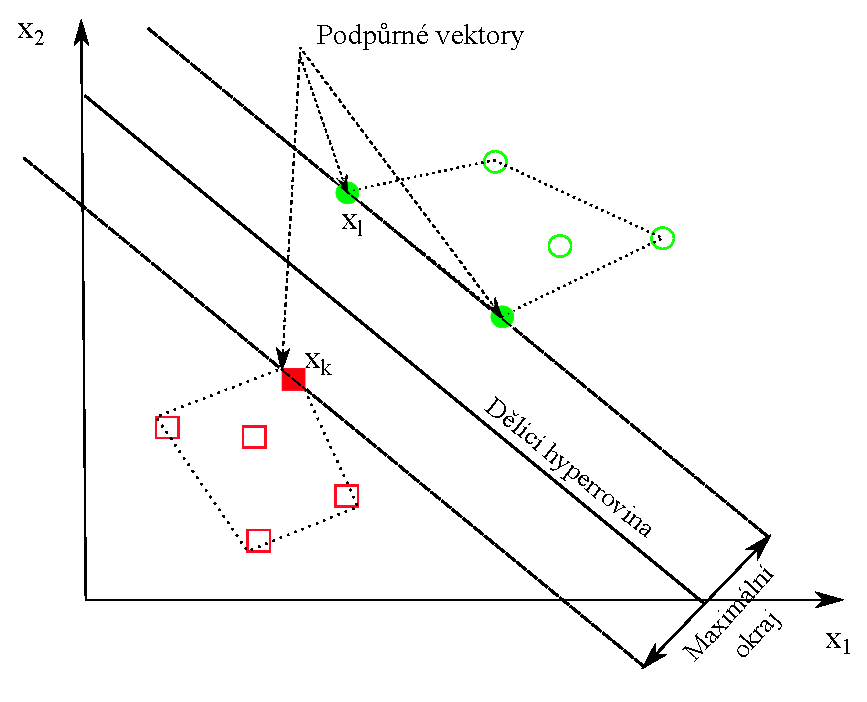
\includegraphics[width=0.63\linewidth]{figures/klasifikace/svm.eps}}
    \caption{Grafické znázornění oddělení vzorků dvou tříd pomocí hyperroviny. Vyplněné body, které tuto hyperrovinu definují, se nazývají podpůrné vektory.}
    \label{fig:svmObrazek}
\end{figure}

\begin{table}[H]
\begin{tabularx}{\linewidth}{>{\parskip1ex}X@{\kern4\tabcolsep}>{\parskip1ex}X}
\toprule
\hfil\bfseries Výhody
&
\hfil\bfseries Nevýhody
\\\cmidrule(r{3\tabcolsep}){1-1}\cmidrule(l{-\tabcolsep}){2-2}

Unikátní řešení\par
Nemá problém tzv. \emph{over-fitting} (česky přetrénování)\par
Velmi účinné\par
Poměrně nízká výpočetní složitost\par
Poskytuje flexibilitu v~možnosti výběru formy prahu
&
Vysoká složitost algoritmu a~s~tím spojená náročnost na pochopení\par
Poměrně pomalé trénování\par
Potíže s~nalezením optimálních parametrů při použití nelineárně odlišitelných dat


\\\bottomrule
\end{tabularx}
\caption{Výhody a~nevýhody metody SVM~\cite{classificMethodsComp2, classificMethodsComp3}.}
\end{table}


\subsection*{Umělé neuronové sítě}
\label{ANN}
Umělá neuronová síť je matematický model inspirovaný biologickými neuronovými sítěmi. Umělá neuronová síť se skládá se ze sekvence vrstev, kde každá vrstva se skládá z~propojené skupiny umělých neuronů a~zpracovává informace za použití přístupu založeného na těchto vazbách. Všechny neurony každé vrstvy jsou váhově spojeny s~neurony předchozí a~následující vrstvy, jak lze vidět na obrázku \ref{fig:ann}. Umělé neuronové sítě slouží pro vytváření složitých vztahů mezi vstupními a~výstupními daty. Úspěšnost těchto sítí závisí zejména na jejich struktuře a~počtu vstupů \cite{classificMethodsComp1, classificMethodsComp3, CVmodernApproach}.

Důležitá podmnožina umělých neuronových sítí pro obor zpracování obrazu jsou konvoluční neuronové sítě popsané samostatně v~kapitole \ref{detekceKonv}.

\begin{figure}[H]
    \centering
    \tmpframe{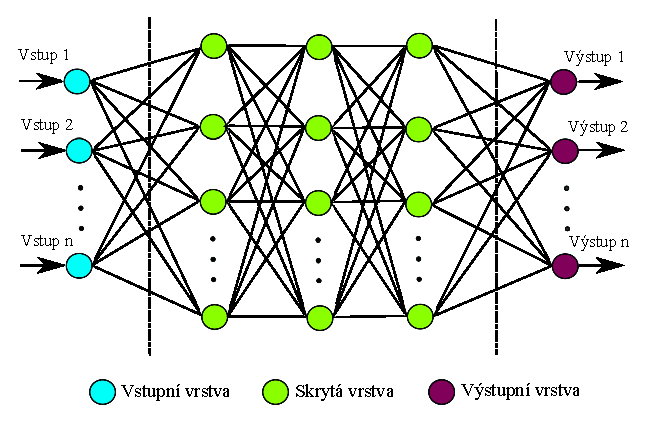
\includegraphics[width=0.70\linewidth]{figures/klasifikace/ann.eps}}
    \caption{Architektura umělé neuronové sítě se třemi skrytými vrstvami. Všechny neurony jsou váhově spojeny se všemi neurony předchozí a~následující vrstvy.}
    \label{fig:ann}
\end{figure}

Učení těchto sítí je možné rozdělit do dvou hlavních tříd:

\begin{itemize}
    \item \textbf{Metoda učení s~učitelem} Funguje na principu anotovaných (oštítkovaných) vstupních dat. Anotace reprezentují správný výsledek pro daný vstup. Pro každý vzorek tedy existuje vektor vstupních dat a~jeden či více očekávaných výsledků. Po provedení klasifikace je výsledek porovnán s~očekávaným výsledkem. Cílem této metody je snížit chybu klasifikace (pomocí ztrátové funkce).
    \item \textbf{Metoda učení bez učitele} se liší oproti metodě s~učitelem v~tom, že vstupní data nejsou vůbec anotovaná, tedy nejsou známy správné výstupy, pomocí kterých by se proces trénování řídil. Tyto sítě pracují na principu třídění vstupních dat na základě jejich podobnosti, bez možnosti ověření správnosti.
\end{itemize}

Většina úloh provádějící rozpoznání vzoru v~oboru zpracování obrazu je řešena pomocí první zmíněné metody učení s~učitelem \cite{CNN}.

\begin{table}[H]
\begin{tabularx}{\linewidth}{>{\parskip1ex}X@{\kern4\tabcolsep}>{\parskip1ex}X}
\toprule
\hfil\bfseries Výhody
&
\hfil\bfseries Nevýhody
\\\cmidrule(r{3\tabcolsep}){1-1}\cmidrule(l{-\tabcolsep}){2-2}

Velmi účinné pro velké datové sady\par
Odolné vůči šumu v~trénovací datové sadě\par
Bez-parametrický přístup. Tzn. nedělá předpoklady o~mapovací funkci\par
Vysoká výpočetní rychlost
&
Vysoká náročnost na výpočetní zdroje a~čas\par
Problém tzv. \emph{over-fitting} (česky přetrénování)\par
Složitost výběru/nalezení správné architektury


\\\bottomrule
\end{tabularx}
\caption{Výhody a~nevýhody umělých neuronových sítí~\cite{classificMethodsComp2, classificMethodsComp3}.}
\end{table}

\subsection*{Rozhodovací stromy}
\label{rozhodovaciStromy}
Rozhodovací strom~\cite{classificMethodsComp2, classificMethodsComp3} vytváří stromovou strukturu jednotlivých rozhodnutí. Rozhodnutí o~členství v~třídě je provedeno pomocí opakovaného rozdělování vstupní datové sady do jednotlivých podmnožin. Je to metoda učení s~učitelem a~oproti umělým neuronovým sítím je bezparametrická. Každá větev graficky znázorňuje rozhodnutí, které by mělo být vykonáno. Metoda umožňuje rozhodnutí o~třídě (akceptaci či odmítnutí) v~libovolném mezikroku a~po provedení klasifikace při trénování rozhodovací stromy udávají sadu pravidel, která by měla být modelem zapamatována. Metoda se skládá ze třech částí. První je rozdělení jednotlivých uzlů, poté následuje nalezení listových uzlů a~nakonec přidělení tříd jednotlivým listovým uzlům.

Metodu rozhodovacích stromů lze ještě dále rozšířit pomocí metody zvané \emph{Random forest} (náhodný les), která během procesu trénování vytváří množinu několika rozhodovacích stromů, kde každý udává (hlasuje pro) třídu vstupního vzorku.

\begin{figure}[H]
    \centering
    \tmpframe{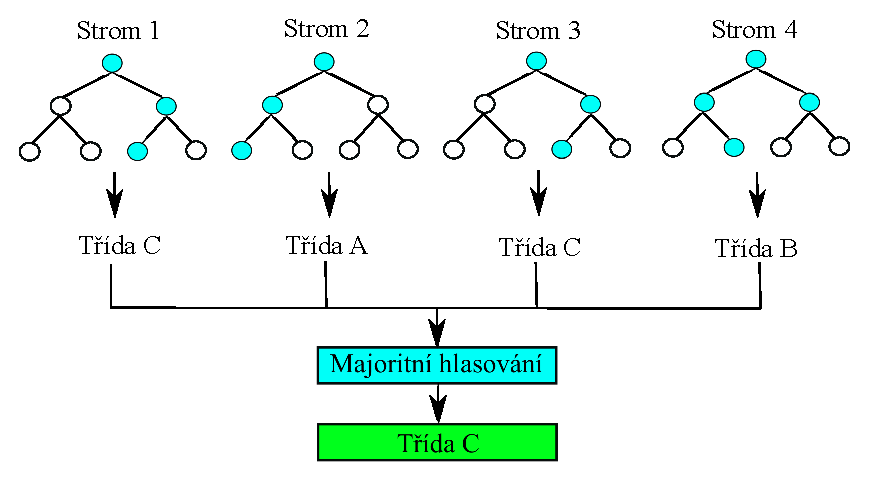
\includegraphics[width=0.7\linewidth]{figures/klasifikace/randomForest.eps}}
    \caption{Náhodný les složený ze čtyř rozhodovacích stromů.}
    \label{fig:rozhodStromy}
\end{figure}

Výsledná třída je určena na základě výsledků jednotlivých rozhodovacích stromů a~to tak, že je vybrána třída s~nejvyšším počtem hlasů \cite{classificMethodsComp1}, znázorněno na obrázku \ref{fig:rozhodStromy}.

\begin{table}[H]
\begin{tabularx}{\linewidth}{>{\parskip1ex}X@{\kern4\tabcolsep}>{\parskip1ex}X}
\toprule
\hfil\bfseries Výhody
&
\hfil\bfseries Nevýhody
\\\cmidrule(r{3\tabcolsep}){1-1}\cmidrule(l{-\tabcolsep}){2-2}

Jednoduché na pochopení\par
Bez-parametrický přístup\par
Nízká výpočetní náročnost
&
Vysoká míra chybovosti klasifikace\par
Rozdělení je velmi citlivé vůči trénovací datové sadě

\\\bottomrule
\end{tabularx}
\caption{Výhody a~nevýhody rozhodovacích stromů~\cite{classificMethodsComp2, classificMethodsComp3}.}
\end{table}



%%%%%%%%%%%%%%%%%%%%%%%%%%%%%%%%%%%%%%%%%%%%%%%%%%%%%%%%%%%%%%%%%%%%%%%%%%%%%%%%%%%%%%%%%%%


\section{Vyhodnocení úspěšnosti detekce}
\label{vyhodnoceniUspesnosti}
Ve chvíli, kdy už existuje funkční model pro detekci objektů, je dobré vyhodnotit jeho úspěšnost. Úspěšnost detekce ve většině případů nestačí vyhodnotit pouhým pozorováním detekovaných obrázků (tedy kvalitativně), ale vyjadřuje se kvantitativně -- proto je potřeba si zavést pojmy, které usnadní validaci detekcí a~určení celkové kvality detektoru. Při studiu této problematiky jsem vycházel z~\cite{mAP}.

\subsection*{Intersection over union -- IoU}
\emph{Intersection over union} (dále jen mezi odborníky běžně používaná zkratka IoU), se počítá na základě dvou ohraničujících boxů -- \emph{ground-truth} (požadovaná výstupní hodnota, dále bude používán jen anglický tvar) -- tedy pozice kde se objekt nachází a~predikce vytvořené detektorem. IoU udává překrytí predikce a~ground-truth normalizované na hodnotu náležící do intervalu $\langle0,1\rangle$. Vizualizováno na obrázku \ref{fig:priou}.

\subsection*{Typy predikcí}
Predikce detektoru jsou rozděleny do čtyř následujících tříd, dále budou požívány pouze jejich zkratky.

\begin{enumerate}
    \item \textbf{True positive} -- Udává správně detekovaný objekt (IoU je větší než hodnota prahu).
    \item \textbf{False positive} -- Udává špatně detekovaný objekt (IoU je menší než hodnota prahu).
    \item \textbf{False negative} -- Udává nedetekovaný objekt.
    \item \textbf{True negative} -- Místa kde není objekt jsou správně označena jako bez-objektová (používá se výjimečně).
\end{enumerate}


\subsection*{Precision}
\emph{Precision} (přesnost, nadále bude využívána jen anglická forma, protože to je zvykem i~mezi odborníky v~oboru), udává, jak přesné predikce jsou. Běžně se uvádí v~procentech a~vyjadřuje kolik z~predikcí je pravdivých:
\begin{align}
    \label{eq:precision}
    \mathrm{Precision} &= \frac{\mathrm{TP}}{\mathrm{TP} + \mathrm{FP}}
\end{align}
\subsection*{Recall}
\emph{Recall} (citlivost, nadále bude využívána jen anglická forma, protože to je zvykem i~mezi odborníky v~oboru), udává, kolik ze všech pozitivních případů bylo správně predikováno:
\begin{align}
    \label{eq:recall}
    \mathrm{Recall} &= \frac{\mathrm{TP}}{\mathrm{TP} + \mathrm{FN}}
\end{align}
\begin{figure}[H]
    \centering
    \tmpframe{\includegraphics[width=0.3\linewidth]{figures/klasifikace/iou.png}}
    \caption{Grafické znázornění IoU pomocí predikovaného a \emph{ground-truth} boxu.}
    \label{fig:priou}
\end{figure}    

\subsection*{Average precision -- AP}
\emph{Average precision} (dále jen mezi odborníky běžně používaná zkratka AP), je metrika používaná pro měření přesnosti detektoru objektů. Udává průměr maximálních hodnotu precision pro různé hodnoty recall. Princip AP je konceptuálně stejný jako počítání plochy pod precision-recall křivkou (AuC -- \emph{area under curve}). První je ale potřeba tzv. vyhladit křivku. Toho se dosáhne interpolací. Vytvoří se graf s~hodnotou recall \Tilde{r} $0.0, 0.1, ... 1.0$ a~každá hodnota precision se nahradí maximální hodnotou precision pro recall $\geq \Tilde{r}$. Graficky znázorněno na obrázku \ref{fig:prcurve}.

\begin{figure}[H]
    \centering
    \tmpframe{\includegraphics[width=0.75\linewidth]{figures/klasifikace/prcurve.png}}
    \caption{Precission-recall křivka a~její interpolace.}
    \label{fig:prcurve}
\end{figure}

AP je počítáno jako průměr maximálních hodnot precision na jedenácti hodnotách recall $(0.0, 0.1, ... 1.0)$. Záměrem interpolace křivky na jedenácti bodech je snížit dopad \uv{zákmitů} křivky, způsobených malými odchylkami hodnocení vzorků. Výpočet je následující:
\begin{align}
    \label{eq:map}
    \mathrm{AP} &= \frac{1}{11} \sum\limits_{r \in \{0.0,...,1.0\}} AP_r\\ &= \frac{1}{11} \sum\limits_{r \in \{0.0,...,1.0\}} p_{i}(r)
\end{align}
kde
\begin{align}
    \label{eq:interpol}
    p_{i}(r) = \max\limits_{\Tilde{r} \geq r} p(\Tilde{r})
\end{align}
Hodnota $p_{i}$ značí interpolovanou precision. AP se počítá pro každou třídu zvlášť, proto se u~detektorů běžně používá mAP (\emph{mean average precision}), což je průměr AP všech tříd.


%%%%%%%%%%%%%%%%%%%%%%%%%%%%%%%%%%%%%%%%%%%%%%%%%%%%%%%%%%%%%%%%%%%%%%%%%%%%%%%%%%%%%%%%%%%


\section{Související práce}
\label{existujiciReseni}
Detekce a~klasifikace dopravních značek je již mnoho let řešená problematika, které spadá do dynamicky rozvíjejícího se oboru detekce objektů v~obraze. Existuje velké množství přístupů k~řešení této problematiky, ale i~přesto detekce značek stále není považována za úplně vyřešenou a~vznikají nové práce, jako je například tato, provádějící detekci za pomoci moderních technik ve snaze posunout tuto problematiku vpřed.

Porovnání výsledků jednotlivých prací není jednoduché, protože se často liší použitými metrikami pro vyhodnocení (hit rate, mAP (interpolovaná), mAP@0.5, mAP@0.75, ROC, F1, atd.). Dalším faktorem při vyhodnocení, který má poměrně velký vliv na celkovou úspěšnost, je použitá datová sada -- datové sady se liší ať už konvencí značek, tak zejména jejich kvalitou a kvantitou. Jejich přehled je možné najít v~sekci~\ref{datoveSady}.

Jak plyne z~porovnání detekčních metod dopravních značek~\cite{tsDetectOverview}, dříve byla tato úloha řešena pomocí segmentace obrazu na základě barvy v~kombinaci s~detekcí geometrických útvarů či rohů~\cite{tsDetect}. V~práci~\cite{fastShapeTSD} se autoři zabývali rychlou metodou detekce tvarů založenou na Houghově transformaci přímo pro detekci dopravních značek. Výsledkem byla $95\,\%$ úspěšnost detekce a~metoda je navíc invariantní vůči natočení značky a~pracuje v~reálném čase.

Metoda hojně využívaná pro detekci značek je extrakce příznaků z~obrazu v~kombinaci s~klasifikátorem. Před příchodem konvolučních neuronových sítí byl přístup s~použitím histogramu orientovaných gradientů (dále jen HOG) v~kombinaci s~SVM (\emph{Support Vector Machines}) označován za tzv. \emph{state of the art}\footnotemark \, detekce objektů~\cite{tsdYolo}. V~práci~\cite{tsdHog} využívající zmíněnou kombinaci HOG a~SVM se podařilo získat na Německé datové sadě výsledky detekce značek s~hodnotami \emph{precision} i~\emph{recall} blížícími se k~jedné, ale vyhodnocení jednoho snímku trvalo déle než vteřinu. Další možností je použití metody využité v~práci~\cite{tsdHaar} -- kombinaci Haarových příznaků s~lineárním SVM pro klasifikaci (a konvolučními neuronovými sítěmi pro verifikaci), pomocí které se podařilo na Německé datové sadě dosáhnout taktéž výsledků s~hodnotami \emph{precision} i~\emph{recall} blížícím se k~jedné a~zároveň zpracování v~reálném čase.

\footnotetext{\emph{State of the art} -- stav techniky (tzn. aktuálně nejlepší způsob pro řešení dané problematiky).}

V~posledních letech přitáhlo velkou pozornost hluboké učení a~standardem pro detekci objektů se tak staly konvoluční sítě. Práce~\cite{rcnn} prokázala, že jejich použití pro detekci objektů může vést ke dramatickému zvýšení úspěšnosti detekce. Výborných výsledků detekce objektů dosáhla metoda R-CNN, která kombinuje návrh kandidátních oblastí (selektivní hledání~\cite{selective-search}) s~konvolučními sítěmi a~řadí se tak do třídy dvou-krokových metod. Upravená verze této metody, Faster R-CNN, byla použita v~práci~\cite{tsdFastRcnn} pro detekci značek a~dosáhla úspěšnosti $34.4\,\%$ mAP na Belgické datové sadě.

Pro rychlejší, ale stále přesnou detekci vznikla třída tzv. \emph{single-shot} detektorů, kam spadá YOLO a~SSD (\emph{Single Shot Detector}). Ty provádí detekci i~klasifikaci pomocí jedné konvoluční sítě. Upravený systém Tiny YOLOv1 byl pro detekci značek použit v~práci~\cite{tsdYolo}, kde se autorům podařilo dosáhnout úspěšnosti $33.8\,\%$ mAP na Belgické datové sadě dopravních značek s~rychlostí 100 snímků za sekundu. SSD byl použit v~práci~\cite{tsdSsd}, kde se autoři snažili o~přesný odhad okrajů dopravních značek a~dosáhli úspěšnosti kolem $85\,\%$ mAP na Německé datové sadě při rychlosti 7 snímků za sekundu na zařízení s poměrně nízkým výpočetním výkonem.

Z~dosažených výsledků zmíněných prací vyplývá, že pro úlohu detekce dopravních značek stále dosahují lepší úspěšnosti systémy využívající extrakci příznaků v~kombinaci s~klasifikátorem, ale konvoluční sítě je pomalu dohánějí jak z~hlediska úspěšnosti, tak rychlosti.